\section{Introduction}
\label{sec:intro}

Task-specific  conversational  chatbot  \cite{wen2016network}  has been applied
into  many practical products. One typical example is the chatbot that shares the working burden of
human  customer  service  agents  responsible  for  customers' questions. 
Another one is intelligent  speakers, e.g. Siri, Google home. 
Regardless of whether these conversations belong to
single or  multi-round, an essential technique underlying this type of chatbot is to
identify  the  real  intention  behind  a  user's  question or reply. 
The detected intention  with  its  associated  information  is then mapped into a
predefined dialog logic graph, from which a suitable response is returned.
This  is  the  main  difference  from  a  free chatbot.  

Intention detection in task-specific chatbot  is  a  challenging task due to its inherent properties. First,
a customer's  utterance  within  a conversation is usually quite short. Since it
does  not  contain  enough  information,  short  texts \cite{song2014short} are
thought  to  be  more  ambiguous  compared to long texts such as paragraphs or
documents,  posing  a  great challenge \cite{chen2019deep} for classification
task   \cite{phan2008learning,yan2009dynamic,hua2015short}.   Second,  in  the
initial  stage  of  building  a  chatbot , it is often rather hard to collect
sufficient  labeled  data  to  train  a good model. Developers have to
examine tons of real system logs for typical user's utterances, and then label
them  with expected intentions. Therefore, to build a task-specific chatbot with
high  performance, it is essential to solve the challenge of short-text
classification   \cite{sriram2010short}   problem   under   few-shot   setting
\cite{yu2018diverse}.


Generally  there  are  two  kinds  of  approaches  to  address  this  problem.


The   first   one,   \emph{text  classification},  includes  classic  long  text
classification   and   short  text  classification  in  this  scenario.  Besides
traditional  machine  learning models like SVM \cite{suykens1999least}, boosting
tree  \cite{tu2005probabilistic},  many work \cite{wen2016network} choose neural
network      such      as      convolutional      neural     networks     (CNNs)
\cite{kim2014convolutional,zhang2015character,conneau2016very}  and  long  short
term  memory  networks  (LSTMs)  \cite{mousa2017contextual,liu2016recurrent}  to
accomplish  the  task  of  extracting  semantic  features from limited amount of
words.  Another two interesting lines of work, label-word
joint models, and joint NER and classification are discussed in the related work
of appendix.  Recently,  pre-trained  language  models  on  large  corpus  like BERT
\cite{devlin2018bert}  and  RoBERTa  \cite{liu2019roberta}  has been proven more
powerful   in   solving  many  NLP  tasks  including  short-text  classification
\cite{madabushi2020cost}.       Especially      for      few-shot      scenarios
\cite{yu2018diverse},     pre-trained     models     based    on    transformers
\cite{vaswani2017attention}  tends to be more helpful to alleviate the dearth of
training data.

The  second  one, \emph{text similarity model}, is usually employed to calculate
how  similar  between an input text and a historical text in the repository. The
associated label of the most similar historical text is returned as the label of
the  text  to  query \cite{jafarpour2010filter,   leuski2011npceditor}.  
A  popular  and  effective  methodology  is adopting BERT
\cite{devlin2018bert} and other pretrained models \cite{liu2019roberta} to model
the similarity model as a binary classification problem.

Despite  the  success  of  these two approaches, they still have some
limitations.  
Regarding  the  \emph{text  classification  model}, when the labeled data in current
domain  is  insufficient,  it  is  quite  hard  to adopt labeled data from other
domains, as their label definitions are often incompatible to each other. Though
we can use some paraphrasing methods, e.g., machine translation based, to expand
the labeled data, the resulting benefit is still limited.
Regarding the  \emph{similarity model}, the foremost advantage is it does not pose
any restriction on label definition in a domain, as it merely models the
similarity of two input texts. Thus, we may borrow plenty of extra data to help
the similarity model training in current domain \cite{sun2019fine}. 
Yet, its biggest disadvantage is its optimization loss differs from that in a
specific task. This always lead to a suboptimal model.  

The  above  limitations motivate us to propose a system that 
takes both the performance of a classification model and the ability of
supporting out-of-domain data from a similarity model.
We call our system as SFC,  short  for  similarity model fused with classification model, shown in
Fig.  \ref{fig:framework}.  We further bring in multi-task learning   \cite{caruana1993multitask,collobert2008unified,  liu2019multi} to train SFC.  
Our basic  idea  consists of two stages. In the first stage, we use an auxiliary model
to  select  top-K most possible labels for an input. This model can be an elastic
search  \cite{divya2013elasticsearch}  or a text classification model trained on
current   task-specific   chatbot   data.  In  the  second  stage,  we  build  a
classification  model  whose  main  modules  are  similarity  models. Then, this
structure  derives  two  goals to train towards, the classification loss for our
application,  and  the similarity loss for the main modules. When the two stages
are  independently optimized, we call \emph{two-stage SFC}. 

We further find that
the  quality of the output from the first stage might limit the final performance of the
system,  since  the  candidate labels for an input is fixed in the
whole  multi-task  training  process.  This  observation motivates us to further
improve  the  two-stage  SFC  into a joint training setting, called \emph{joint SFC}. In
this  way,  the  candidate texts associated  with the top-K classes also become
dynamic,  and  the  text  classification  model  in the first stage will also be
further optimized to provide better top-K results by the final training loss.

Experiment  results  from  4  public  and  1  private  short-text classification
datasets,  show  that  our proposed SFC joint system can achieve significant and
consistent  improvements  over  strong baselines, especially in the low resource
settings.

\begin{figure*}[t]
  \begin{centering}
    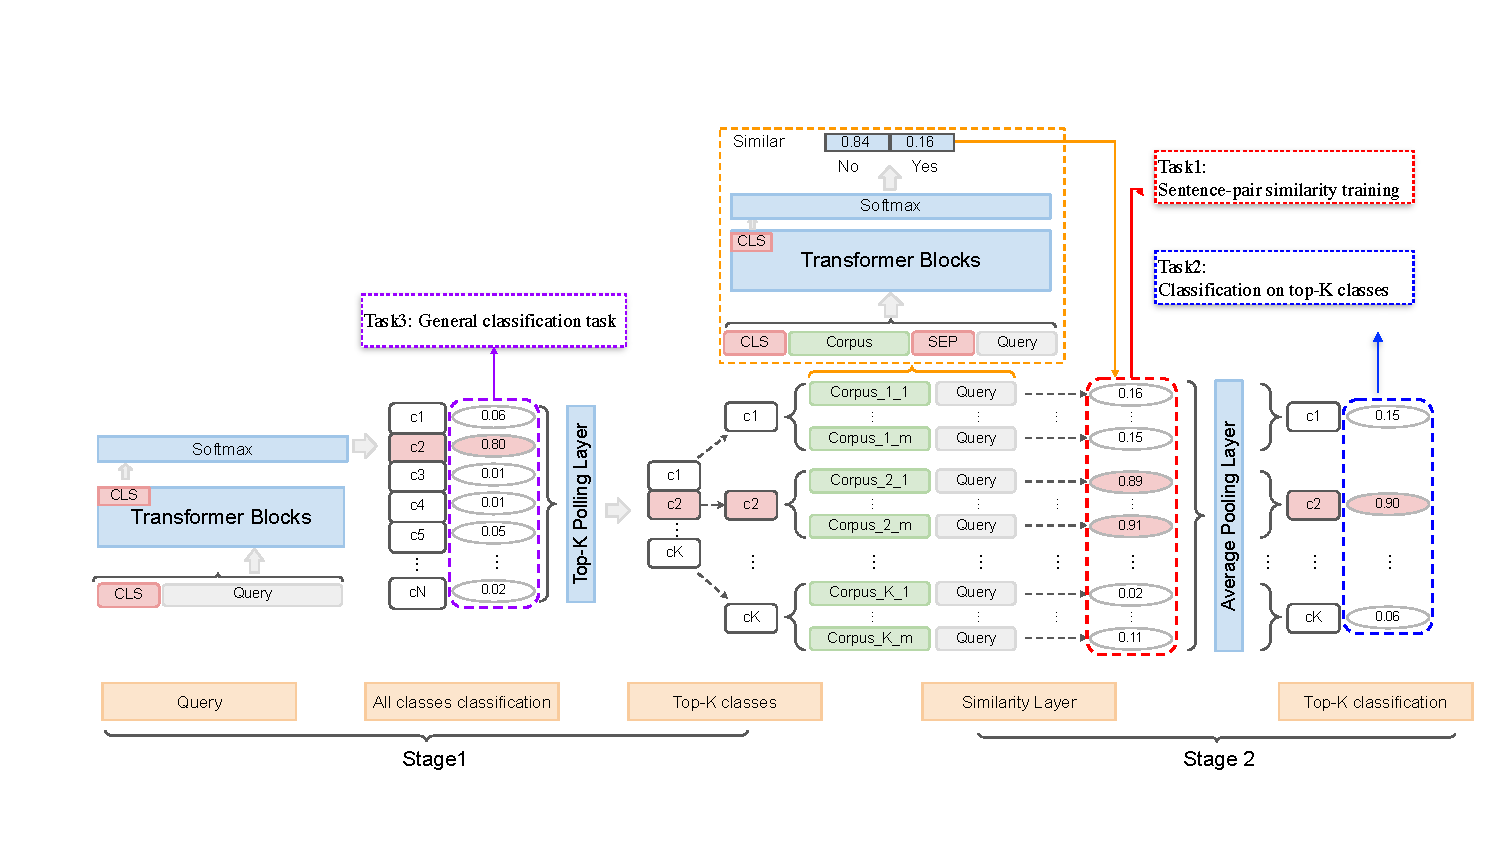
\includegraphics[scale=0.66]{picture/picture4} 
    \par
  \end{centering}
  \caption{
    \textbf{Network Structure of SFC:} two-stage SFC and joint-SFC are sharing
    the  same  network  from  stage  1  and  stage 2, with the only difference
    whether two stages being jointly trained.
  }
  \label{fig:framework}
\end{figure*}

